\documentclass[10pt]{beamer}

\usepackage{amssymb,amsmath}
\usepackage{graphicx}
\usepackage{url}
\usepackage{color}
\usepackage{pagenote}[continuous,page]
\usepackage{relsize}		% For \smaller
\usepackage{url}			% For \url
\usepackage{epstopdf}	% Included EPS files automatically converted to PDF to include with pdflatex

%For MindMaps
% \usepackage{tikz}%
% \usetikzlibrary{mindmap,trees,arrows}%

%%% Color Definitions %%%%%%%%%%%%%%%%%%%%%%%%%%%%%%%%%%%%%%%%%%%%%%%%%%%%%%%%%
%\definecolor{bordercol}{RGB}{40,40,40}
%\definecolor{headercol1}{RGB}{186,215,230}
%\definecolor{headercol2}{RGB}{80,80,80}
%\definecolor{headerfontcol}{RGB}{0,0,0}
%\definecolor{boxcolor}{RGB}{186,215,230}

%%% Save space in lists. Use this after the opening of the list %%%%%%%%%%%%%%%%
%\newcommand{\compresslist}{
%	\setlength{\itemsep}{1pt}
%	\setlength{\parskip}{0pt}
%	\setlength{\parsep}{0pt}
%}

%\setbeameroption{show notes on top}

% You should run 'pdflatex' TWICE, because of TOC issues.

% Rename this file.  A common temptation for first-time slide makers
% is to name it something like ``my_talk.tex'' or
% ``john_doe_talk.tex'' or even ``discrete_math_seminar_talk.tex''.
% You really won't like any of these titles the second time you give a
% talk.  Try naming your tex file something more descriptive, like
% ``riemann_hypothesis_short_proof_talk.tex''.  Even better (in case
% you recycle 99% of a talk, but still want to change a little, and
% retain copies of each), how about
% ``riemann_hypothesis_short_proof_MIT-Colloquium.2000-01-01.tex''?

\mode<presentation>
{
  \usetheme{CambridgeUS}
  \usecolortheme{dolphin}
  \useoutertheme{default}
  \useinnertheme{default}
  \setbeamercovered{invisible} % or whatever (possibly just delete it)
}
\beamertemplatenavigationsymbolsempty

\usepackage[english]{babel}
%\usepackage[latin1]{inputenc}
\usepackage{subfigure}

\usepackage{times}
\usepackage[T1]{fontenc}
\usepackage{CJKutf8}

%% makes the ppagenote command for figure references at the end.
\makepagenote
\renewcommand{\notenumintext}[1]{}
\newcommand{\ppagenote}[1]{\pagenote[Page \insertframenumber]{#1}}

\title[Experiment Design (01CH740)]{Experiment Design for Computer Sciences (01CH740)}
\author[Claus Aranha]{Claus Aranha\\{\footnotesize caranha@cs.tsukuba.ac.jp}}
\institute[U. Tsukuba]{University of Tsukuba, Department of Computer Sciences}


% TODO: Topics for this class
% TODO: Basic statistical concepts: mean, median, quantile, variance
% TODO: Basic statistical concepts: Boxplot, histograms, how to observe data
% TODO: Basic statistical concepts: QQ plot to compare two distributions
% TODO: Basic R concepts: Reading data, summary, plotting, functions
% TODO: Basic R concepts: examining a data set (example 1,2,3)
% TODO: Class overview: practical data exploration, theory starts on class 4
% TODO: Statistical reviews: Normal, T, etc


\title[]{Experiment Planning and Design}
\subtitle[]{Lecture 3: Experimental Statistics}
\author[Claus Aranha]{Claus Aranha\\{\footnotesize caranha@cs.tsukuba.ac.jp}}
\institute{Department of Computer Science}
\date{2015-04-29}

\begin{document}

\section{Introduction}
\subsection{Outline}

\begin{frame}
  \maketitle
\end{frame}

\begin{frame}
  \frametitle{Before we begin} 

  \begin{block}{Homework Feedback}
  Last week I asked you all for a simple description of your projects,
  and how you would expect to use experiments in these projects. Let's
  take a look at the responses and do some comments.
  \end{block}

\end{frame}

\begin{frame}
  \frametitle{Class Outline}
  \begin{block}{}
    In this class, we will start to look at the statistical and
    technical tools that are used when designing, preparing and
    analysing data and experiments.
  \end{block}
  \begin{block}{}
    These topics are generic enough that they should be useful for all
    of you, but each of these techniques can (and has!) been refined
    to deal with different, specific situations.
  \end{block}

  \bigskip

  \begin{itemize}
  \item Why to statistically analyze data?
  \item Simple ``R'' tutorial;
  \item Statistical Indicators
  \item Hypothesis testing
  \end{itemize}
\end{frame}

\subsection{Motivation}

\begin{frame}
  \frametitle{The Story of Alice and Bob}
  \begin{block}{}
    Alice and Bob are two competing scientists.
    \bigskip
    Each has developed a new program that minimizes the number of spam
    messages that a person receives in their inbox everyday.
    \bigskip
    They decide to compare their approaches to decide which one is
    better.
  \end{block}
\end{frame}

\begin{frame}
  \frametitle{The Story of Alice and Bob (2)}
  \begin{block}{}
    Alice and Bob test their programs. They create a mail account, and
    count the number of spam e-mails that is received in a one-day
    period, using their software. 
  \end{block}
  \begin{block}{}
    After the test, Bob claims that his software is the best. Is he
    correct? Why?
  \end{block}
  \begin{columns}[c]
    \column{0.5\textwidth}
    \begin{tabular}{c|c}
      Alice & Bob \\
      \hline\\
      9.533777 & 7.132107
    \end{tabular}
    \column{0.5\textwidth}
    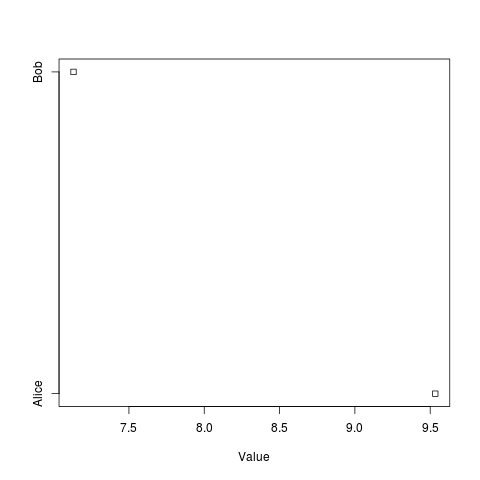
\includegraphics[width=.7\textwidth]{img/AliceBob_1}
  \end{columns}
\end{frame}

\begin{frame}
  \frametitle{The Story of Alice and Bob (3)}
  \begin{block}{}
    Alice complains, and says that Bob created his e-mail account a
    few hours later than her (he didn't). They decide to repeat the
    test the next day.

    \medskip

    This time Alice's software not only catch all spam, it also
    catches some annoying chain mails from grandma that the user did
    not want either!
  \end{block}
  \begin{columns}[c]
    \column{0.5\textwidth}
    \begin{tabular}{c|c}
      Alice & Bob \\
      \hline\\
      9.533777 & 7.132107\\
      -8.149627 & 3.689753\\
    \end{tabular}
    \column{0.5\textwidth}
    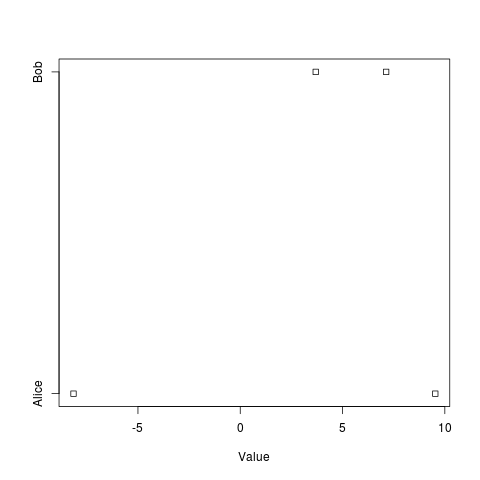
\includegraphics[width=1\textwidth]{img/AliceBob_2}
  \end{columns}
\end{frame}

\begin{frame}
  \frametitle{The Story of Alice and Bob (4)}
  \begin{block}{}
    Alice and Bob do the experiment for three more days. After five
    total days, Alice claims that on average, her program receives less
    spam than Bob's, and is the better program.

    \smallskip

    \alert{Is she right? Can you comment on their experiment?}
  \end{block}
  \begin{columns}[c]
    \column{0.5\textwidth}
    \begin{tabular}{c|c}
      Alice & Bob \\
      \hline\\
      9.533777 & 7.132107\\
      -8.149627 & 3.689753\\
      8.55298 & 13.951185\\
      8.105736 & 10.098746\\
      10.879449 & 7.59397\\
      \hline
      \hline\\
      Mean & Mean\\
      5.784463 & 8.493152\\
    \end{tabular}
    \column{0.5\textwidth}
    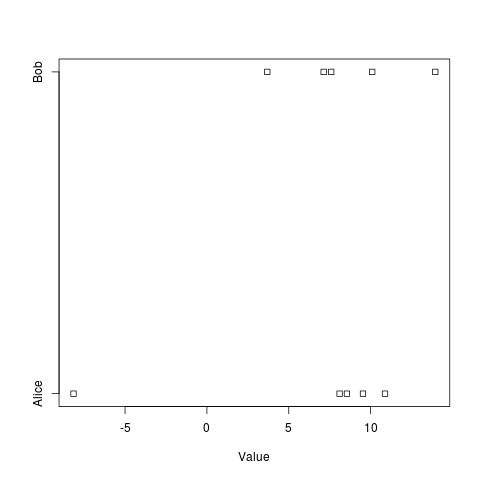
\includegraphics[width=1\textwidth]{img/AliceBob_5}
  \end{columns}
\end{frame}

\begin{frame}
  \frametitle{The Story of Alice and Bob (5)}
  \begin{block}{}
    If we make a few more experiments, the difference between the
    means becomes really small. Is this the correct value? How do we
    know when to stop making experiments?
  \end{block}
  \begin{columns}[c]
    \column{0.5\textwidth}
    {\small
    \begin{tabular}{c|c}
      Alice & Bob \\
      \hline\\
      9.533777 & 7.132107\\
      -8.149627 & 3.689753\\
      8.55298 & 13.951185\\
      8.105736 & 10.098746\\
      10.879449 & 7.59397\\
      12.482068 & 5.179808\\
      12.992992 & 7.030863\\
      11.022459 & 14.178277\\
      6.454991 & 8.728171\\
      13.055410 & 7.806157\\      
      \hline
      \hline\\
      Mean & Mean\\
      8.493023 & 8.538904\\
    \end{tabular}}
    \column{0.5\textwidth}
    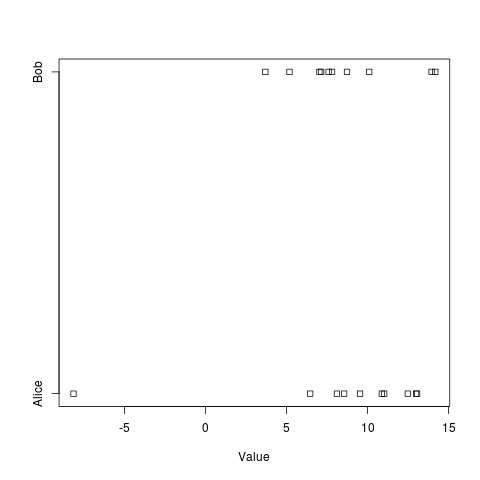
\includegraphics[width=1\textwidth]{img/AliceBob_10}
  \end{columns}
\end{frame}

\begin{frame}
  \frametitle{The Story of Alice and Bob -- Conclusion}
  \begin{block}{}
    In reality, the values for the experiments of Alice and Bob came
    from the same distribution. This means that their technologies are
    equal, and any differences were only luck.
  \end{block}
  \bigskip
  
  \begin{itemize}
  \item Using statistical techniques, we can answer the questions:
    \begin{itemize}
    \item Are these two groups of values REALLY different?
    \item If they are different, HOW MUCH are they different?
    \end{itemize}
  \item We will apply those techniques using the tool ``R''
  \end{itemize}
\end{frame}

\begin{frame}
  \frametitle{The takeaway message} 

  Our monkey-brains are \alert{very bad} at seeing the big
  picture. 
  
  \bigskip
  
  Our intelligence is optimized for pattern matching and, thus, we
  tend to quickly grab the first interpretation that jumps to the eye.

  \bigskip
  
  Statistics is a great tool to make sense of data in ways that may
  not be immediately obvious.

  \bigskip
  
  
\includegraphics[width=0.6\textwidth]{img/smile}

\end{frame}

\section{Introduction to R}
\subsection{What is R?}

\begin{frame}
  \frametitle{The statistical package ``R''}
  \begin{center}
    
\includegraphics[height=0.2\textheight]{img/rlogo}
    \hfill
    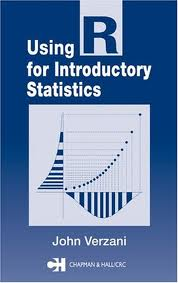
\includegraphics[height=0.3\textheight]{img/rintrobook}
  \end{center}
  \bigskip
  
  \begin{itemize}
  \item Open-Source (GNU) language for statistical computing;
  \item \url{http://www.r-project.org};
  \item Developed since 1990
  \item ``Using R for Introductory Statistics'' by John Verzani
  \end{itemize}
\end{frame}

\begin{frame}[singeslide,fragile]
  \frametitle{Getting Started} 
  
  First, let's install the library from the ``Using R'' book.\\(This can be
  used to install other libraries as well)

  \begin{block}{Install the package from the Internet}
\begin{verbatim}
> install.packages("UsingR")
\end{verbatim}
  \end{block}

  \begin{block}{Load Library after installation}
\begin{verbatim}
> library(UsingR)
\end{verbatim}
  \end{block}
\end{frame}

\subsection{R Basics}
\begin{frame}[singleslide,fragile]
  \frametitle{Basic R Commands}
  \begin{block}{}
    R works as a commandline program. You enter commands and get their
    results. For example, we can use R as a simple calculator, by
    trying out the following commands, and pressing <ENTER>
  \end{block}
\bigskip

\begin{verbatim}
> 2 + 2

> 4^8

> 4**8
\end{verbatim}
\end{frame}
\begin{frame}[singleslide,fragile]
  \frametitle{Basic R commands (2)}
  \begin{block}{}
    \structure{Functions} are very important for R. You can specify
    parameters for the functions, or use default values.
  \end{block}
\begin{verbatim}
> factorial(10)
> sin(pi)

> log(27)
> log(27,3)
> log(base=3,27)

> squareroot(2)
> sqrt(-2)  
\end{verbatim}
\medskip

In the last example, we got a nice error message! Error messages can
be \alert{Errors} or \structure{Warnings}
\end{frame}

\begin{frame}[singleslide,fragile]
  \frametitle{Basic R commands (3)}
  \begin{block}{Assigning Variables}
\begin{verbatim}
> x = 3
> x <- 3
> x -> 3
\end{verbatim}
\medskip
  \end{block}
  \medskip

  \begin{block}{}
    Names can be letters, numbers and a period.
    \alert{Case is important!}
\begin{verbatim}
> x = 3
> X = 4
> x + 1
\end{verbatim}
  \end{block}
\end{frame}

\subsection{Working with Arrays}

\begin{frame}[singleslide,fragile]
  \frametitle{Arrays in R}
  \begin{block}{}
    In statistical analysis, we usually work with many values: tables
    or arrays. For example, data sets or experiment results.
  \end{block}
  \bigskip

\begin{verbatim}
Creating an array in R:
> a = c(1,2,3,4)
> a

> b = c("alpha", "beta", "gama")
> b

Be careful! Each array can only have on type!
> c = c("one", 2, "three")
\end{verbatim}
\end{frame}

\begin{frame}[singleslide,fragile]
  \frametitle{Functions and Arrays}
  \begin{block}{Many functions in R accept arrays as data}
\begin{verbatim}
> x = c{1,2,3,4,5,6}
> factorial(x)
> sqrt(x)
> log(x)
> x+x
> x*3
\end{verbatim}
  \end{block}

  \begin{block}{There are also many array specific functions}
\begin{verbatim}
> sum(x)
> mean(x)
> len(x)

Also max(),min(),range(),sort(),cumsum(),diff() ...
\end{verbatim}
  \end{block}
\medskip
\end{frame}

\begin{frame}
  \frametitle{POP QUIZ!}

  \begin{block}{Calculate the Standard Error of this data:}
    10,11,12,13,12,11,10,11,12,13
  \end{block}
  \medskip

  Answer:
  \smallskip

  \begin{onlyenv}<2>
    c=(10,11,12,13,12,11,10,11,12,13)\\
    error = sqrt(sum((mean(x) - x)**2)/length(x))
  \end{onlyenv}
\end{frame}

\begin{frame}[singleframe,fragile]
  \frametitle{Accessing Arrays}
  \begin{block}{We can use numbers or arrays to access particular numbers}
\begin{verbatim}
> x = c(2,4,6,8,10,12)
> x[2]
> x[c(1,2,3)]
\end{verbatim}
  \end{block}
  \begin{block}{Some cool ways to access arrays}
\begin{verbatim}
> 1:3
> x[1:3]
> x[(1:3)*2]
> x[3:1]

> x > 7
> x[x>7]
\end{verbatim}
  \end{block}
\end{frame}

\subsection{Getting Help}
\begin{frame}[singleframe,fragile]
  \frametitle{Listing and Saving your work}

\begin{block}{List all variables that exist in the environment}
\begin{verbatim}
> ls()
or
> objects()
\end{verbatim}
\end{block}

\begin{block}{Saving the work done so far}
\begin{verbatim}
> dump(ls(),file="variables.R")
> dump(c(x,y,result),file="xy.txt",append=TRUE)
\end{verbatim}
\end{block}

\begin{block}{Reading a file with R commands}
\begin{verbatim}
> source("variables.R")
> source("xy.txt")
\end{verbatim}
\end{block}
\end{frame}

\begin{frame}[singleframe,fragile]
  \frametitle{Getting Help}

\begin{verbatim}
> help()               # main help window
> help(``topic'')      # help for ``topic''
> help(mean)       # help for an specific function

> ??''topic''          # keyword search for ``topic''
> help.search("mean")

> help.start()         # Open help in browser

> example(mean)        # Executes an example for the function!
\end{verbatim}
\end{frame}

%% TODO: add exercises?
\begin{frame}
  \begin{center}
    Questions before we move on?\\
    Play a bit with what we have seen so far!
  \end{center}
\end{frame}

\section{Data Analysis}
\subsection{Data Analysis}
\begin{frame}
  \frametitle{Data Analysis}
  \begin{center}
    {\it Before you begin experimenting, take a hard, long look at the
      data.}
  \end{center}
\end{frame}

\begin{frame}
  \frametitle{First step of the experiment workflow}
  \begin{itemize}
    \item By examining the data, we can learn many things about our
      problem, before we even do any experiments;
      \begin{itemize}
      \item (Difficulty of the problem, dimensionality, desired values,
        hard cases, easy cases, problematic factors, etc)
      \end{itemize}
    \item Data examination can be textual, or graphical;
    \item Very important for Optimization, Signal analysis, Field
      studies. (Important in other fields as well)
  \end{itemize}
  \begin{block}{When to visualize data}
    \begin{itemize}
    \item Before the experiment: Investigate dataset properties;
    \item After the experiment: Investigate results;
    \end{itemize}
  \end{block}
\end{frame}

\subsection{Data Frames}

\begin{frame}[singleslide, fragile]
  \frametitle{Data in R: Frames}
  \begin{block}{}
    Multivariate data in R is stored in \structure{data frames}. Think
    of these frames as matrices, where each row is a different data
    point (experiment, sample), and each columns is a different
    parameter or factor.
  \end{block}
\medskip

\begin{verbatim}
> x = c{"Alice","Alice","Alice","Bob","Bob","Bob")
> y = c(8,-8,7,7,3,6)
> t = data.frame(x,y)
# Warning! X and Y must be of the same length!

> names(t) = c("Experimenter","Test Result") 
# What does this do?

> z = c(20,30,20,10,40,20)
> t = data.frame(x,y,z)
\end{verbatim}
\end{frame}

\begin{frame}[singleslide, fragile]
  \frametitle{Loading Frames from disk}
  \begin{itemize}
  \item You can read a data frame into R by using the \structure{read.table()} command. 
\begin{verbatim}
> t = read.table(fnet.txt)
# Warning! If loading a big table, don't forget to
# Assign a variable :-)
\end{verbatim}
\medskip

  \item There are many parameters in this command, such as separator
    character, and whether to use headers or not.
\medskip

  \item The default parameters expect a data file like this:
\begin{verbatim}
10 15 30
30 10 10
40 5  30
70 1  10
\end{verbatim}
  \end{itemize}
\end{frame}

\begin{frame}[singleslide,fragile]
  \frametitle{Accessing Data}
  \begin{itemize}
  \item We can access an item in a Data frame using the notation:
    \structure{frame[row,column]};
{\small
\begin{verbatim}
> AB = read.table("AliceBob.table",header = TRUE)
> AB[1,2]
> AB[,2]
> AB[1,]
> AB[1:10,2]
\end{verbatim}}

  \medskip 
  \item We can also \structure{attach} a frame, and access the columns
  by name;
{\small
\begin{verbatim}
> attach(AB)
> names(AB)
> Value
> AB[Researcher=="Alice",]
> AB[Value > 8,]

# Be careful! Attached variables don't change the main table!
> Value[3] = 5
> AB[3,] # Did not change!
\end{verbatim}}
  \end{itemize}
\end{frame}

\subsection{Textual Analysis}

\begin{frame}
  \frametitle{Textual Analysis of the Data}
  \begin{block}{Things to ask yourself}
    \begin{itemize}
    \item What are the ranges of the factors?
    \item What are the means and the medians? 
    \item What is the ``shape'' of the data?
    \end{itemize}
  \end{block}
  \medskip
  \begin{center}
    This is important for both the problem data set, and for the
    analysis of the results!
  \end{center}
\end{frame}

\begin{frame}[fragile,singleslide]
  \frametitle{Getting Data from the Data}
  \begin{block}{}
\begin{verbatim}
## Loading the data and examining the columns
> Test = read.table("fnet.data", header = TRUE)
> names(Test)
> attach(Test)

## Finding the limits
> range(M)
> range(Depth)
> mean(M)
> median(M)
\end{verbatim}
  \end{block}
  
  \begin{itemize}
  \item When is the mean different from the median?
  \item ``Half of all people are below the mean'' - true or false?
  \end{itemize}
\end{frame}

\begin{frame}[fragile,singleslide]
  \frametitle{More Data commands!}
  \begin{block}{}
\begin{verbatim}
# Loading a smaller dataset: "kid.weights"
> library(UsingR)
> name(kid.weights)

# stem tells us the "shape" of the data
> stem(age); stem(height); stem(weight)

# quantiles of the data
> quantile(height)
> quantile(M)
> IQR(M) # Distance between 2nd and 3rd quartiles

# List of all "Factor Levels"
> table(Mo)
> summary(kid.weights)
\end{verbatim}
  \end{block}
\end{frame}


\subsection{Graphical Visualization}

\begin{frame}
  \frametitle{One image is worth more than 1000 data points}
  \begin{block}{We can use R to plot many different data plots!}
    \begin{itemize}
    \item Central Tendency
    \item Modality
    \item Skew
    \item Distribution
    \item Outliers
    \end{itemize}
  \end{block}
\end{frame}

\begin{frame}[singleslide,fragile]
  \frametitle{Before we begin}
  \begin{block}{}
    R has a large array of ``output devices'': to the screen, png
    files, pdf files, etc. The default is outputting to the screen,
    but that is not good for old computers.
  \end{block}
\bigskip

\begin{verbatim}
> png() # change the output device to png
> dev.cur() # list the current devices

# To get more information
> ?Devices # list many, many devices
\end{verbatim}
\end{frame}

\begin{frame}[fragile,singleslide]
  \frametitle{Data Visualization}
    \begin{block}{Histograms}
      {\small
        \begin{itemize}
        \item Can show the probability distribution of a variable with
          great detail;
        \item Best for samples with large number of observations;
        \item Size of the ``bins'' can be adjusted to increase/decresar
          resolution;
      \end{itemize}}
    \end{block}
    \small{
\begin{verbatim}
> hist(heights)
> hist(weights, labels=TRUE, col="blue")
\end{verbatim}}
\medskip

\begin{center}
  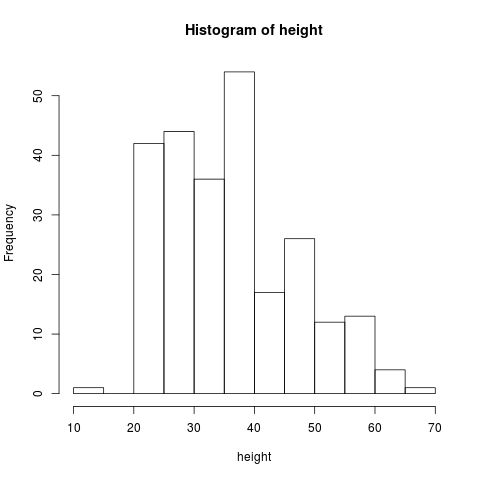
\includegraphics[width=0.25\textwidth]{img/hist01}\hspace{0.2\textwidth}
  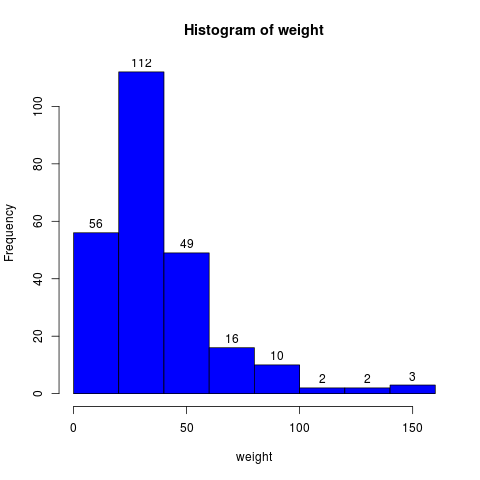
\includegraphics[width=0.25\textwidth]{img/hist02}
\end{center}
\end{frame}

\begin{frame}[fragile,singleslide]
  \frametitle{DataVisualization (2)}
  \begin{block}{Scatterplots}
    For data with two variables, a scatterplot is a good place to
    begin the data analysis.
  \end{block}
  \begin{columns}[c]
   \column{0.6\textwidth}
   \small{
\begin{verbatim}
> png()
> quake = read.table("fnet.txt",
                     header=TRUE)
> attach(quake)
> plot(M,Depth)
> dev.off()
\end{verbatim}}
\column{0.4\textwidth}
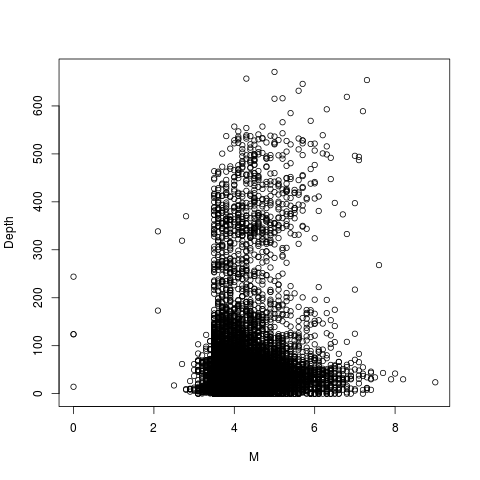
\includegraphics[width=1\textwidth]{img/scatter.png}
\end{columns}

\end{frame}

\begin{frame}[fragile,singleslide]
  \frametitle{Data Visualization (3)}
  \begin{block}{Point Diagram}
    If you want to compare the same value over different classes, a
    stripchart will be useful.
    \medskip

    Let's try to see Alice's and Bob's story again!
  \end{block}
  \begin{columns}[c]
    \column{0.6\textwidth}
\tiny{
\begin{verbatim}
## Many small tricks in this one -- check all the help files!
> AB = read.table("AliceBob.table",header=T)
> attach(AB)
> AB.means = tapply(Value,Researcher,mean)
> stripchart(Value~Researcher, xlab=expression("Flying Distance"), 
             pch=16, cex=1.2,cex.axis=1.5)
> arrows(AB.means,c(1.3,1.7), AB.means,c(1,2),length=.1)
> text(AB.means,c(1.2,1.8),round(AB.means,2),pos=4,cex=2)
\end{verbatim}}
    \column{0.4\textwidth}
    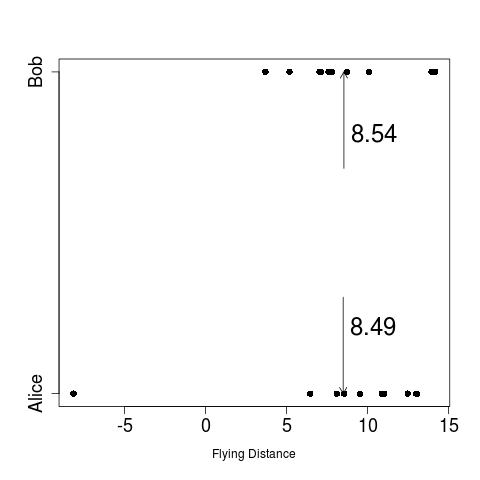
\includegraphics[width=1\textwidth]{img/point.png}
  \end{columns}
\end{frame}

\begin{frame}[fragile,singleslide]
  \frametitle{Data Visualization (4)}
  \begin{block}{Box Plots}
    Very important for understanding multi-variate data:
    \begin{itemize}
      \item Can be used for various sample sizes;
      \item Gives an idea of the distribution of the data;
      \item Can be used for multiple factors at the same time;
    \end{itemize}
  \end{block}
  \begin{columns}[c]
    \column{0.6\textwidth}
\small{
\begin{verbatim}
> library(UsingR)
> png()
> attach(ewr)
> boxplot(AA,CO,DL,HP,NW,TW,US)
> dev.off()
\end{verbatim}}
    \column{0.4\textwidth}
    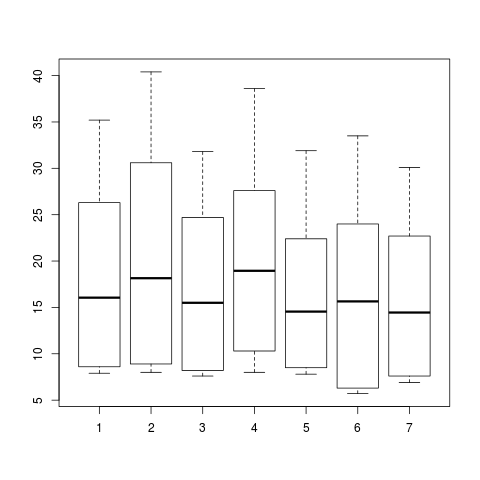
\includegraphics[width=1\textwidth]{img/boxplot}
  \end{columns}
\end{frame}

\begin{frame}[fragile,singleslide]
  \frametitle{Data Visualization (5)}
  \begin{block}{QQ Plot}
    \begin{itemize}
    \item Compares the quantiles of two samples
    \item Allow you to compare the shapes of two distributions
    \item For example, you can compare the shape of a normal
      distribution with the shape of your data.
    \end{itemize}
  \end{block}
\small{
\begin{verbatim}
> qqnorm(M)
> qqnorm(Value)
> qqnorm(Value[Value > 0])
\end{verbatim}}
\begin{center}
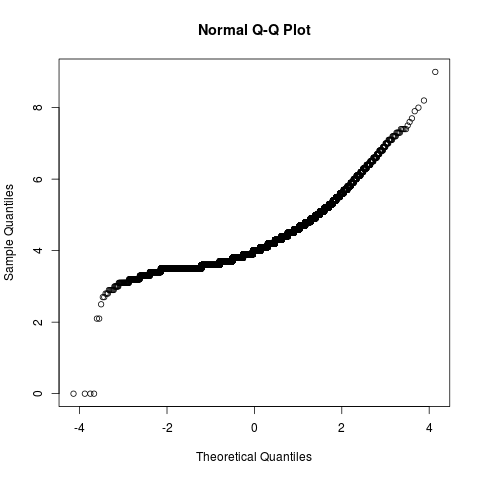
\includegraphics[width=0.25\textwidth]{img/qqplot1}\hspace{0.1\textwidth}
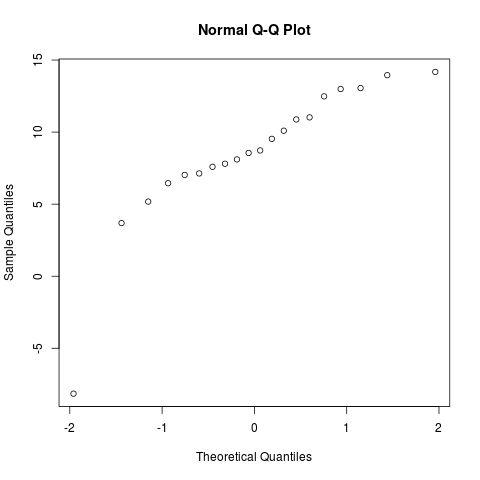
\includegraphics[width=0.25\textwidth]{img/qqplot2}\hspace{0.1\textwidth}
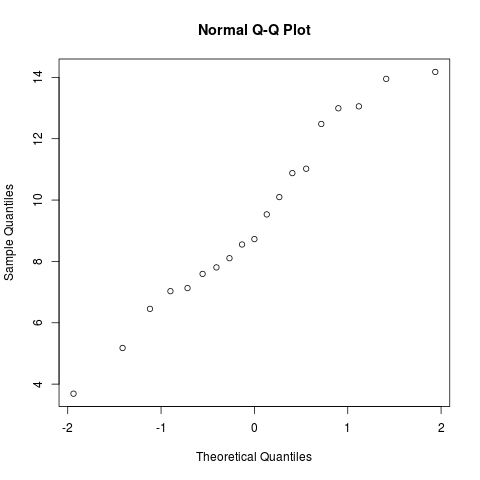
\includegraphics[width=0.25\textwidth]{img/qqplot3}
\end{center}
\end{frame}

\begin{frame}
  \frametitle{This is NOT all}
  \begin{block}{}
    There are many, many different ways of presenting and graphically
    analyzing data. This just scratches the surface! We might see a
    few more during this course, but you should also look for examples
    online and read manuals and FAQs.
  \end{block}

  \begin{block}{}
    Now let us talk about \structure{Scientific Hypothesis}
  \end{block}
\end{frame}

\section{Hypothesis Testing}
\begin{frame}
  \frametitle{}
\end{frame}

%%%%%%%%%%%%%%%%%%%%%%%%%%%%%%%%%%%%%
%% Still the Same as intensive course
%% Needs re-writing

\section{Distributions and Intervals}
\subsection{Theory}

\begin{frame}
  \frametitle{Plato and his Cave}
  \begin{block}{Population}
    \begin{itemize}
    \item ``Population'' regards all the possible values for a variable;
    \item Usually it is impossible to directly observe;
    \end{itemize}
  \end{block}
  \begin{block}{Sample}
    \begin{itemize}
    \item ``Sample'' are the values for the variable observed in an experiment;
    \item It is a subset, drawn from the population;
    \end{itemize}
  \end{block}

  \medskip

  \begin{onlyenv}<2>
    \begin{block}{}
      In an statistical analysis, we want to discover information
      about the population, by extrapolating from the sample we got
      from the experiment.
    \end{block}
  \end{onlyenv}
\end{frame}

\begin{frame}
  \frametitle{Sampling and Sampling Distributions (1)}
  \begin{block}{}
    Statistical Inference: Making conclusions about a population from
    a sample taken from this population.
  \end{block}
  \bigskip

  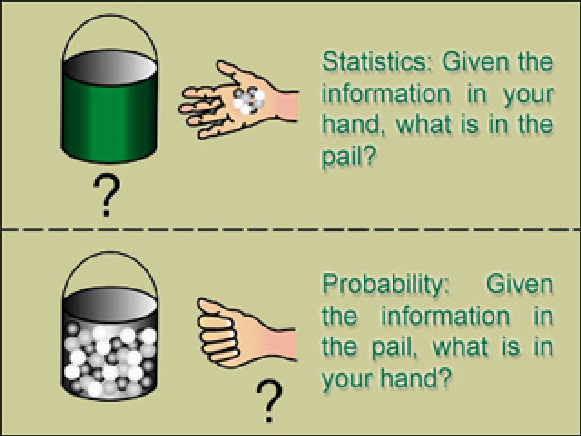
\includegraphics[width=0.6\textwidth]{img/sampleandpopulation}
\end{frame}

\begin{frame}
  \frametitle{Sampling and Sampling Distributions (2)}
  \begin{block}{Some more concepts}
    \begin{itemize}
      \item \structure{Degrees of Freedom}: Number of Independent
        factors, or sources of variation in a given statistic
        (parameters)
      \item \structure{Distributions}: Description of the sample (or
        population)
        \begin{itemize}
        \item Normal;
        \item Power Law;
        \item $\chi^2$
        \item $t$
        \item $F$
        \item etc.
        \end{itemize}
    \end{itemize}
  \end{block}
\end{frame}

\subsection{R Tools}
\begin{frame}
  \frametitle{Creating a Sample (and analyzing it)}
  \begin{itemize}
  \item The ``sample()'' command;
  \item Mean, Variance, Standard Deviation; -- now with different meanings
  \item Z-scores;
  \item Correlation (and spearman rank)
  \end{itemize}
\end{frame}

\begin{frame}
  \frametitle{Distributions in R}
  \begin{block}{The d, p, q, r family}
    \begin{itemize}
    \item d: probability distribution function
    \item p: cumulative distribution function
    \item q: quantiles
    \item r: random samples
    \end{itemize}
  \end{block}
  \begin{block}{Some sample distributions}
    unif, binom, norm, exp, lnorm, etc...
  \end{block}
\end{frame}


\subsection{The Central Limit Theorem}
\begin{frame}
  \frametitle{Central Limit Theorem}
  \begin{block}{}
    Let $y_1,...,y_n$ a series of random variables with mean $\mu$ and
    variance $\sigma^2$ finites, and let $x = \sum y_i$. Then:
    \begin{equation}
      Z_n = \frac{x - n\mu}{\sqrt{n\sigma^2}}
    \end{equation}
    can be approximated to a normal(0,1) distribution.
  \end{block}
  
  \bigskip

  \structure{What does this mean?}\\ 
  When the error in an experiment is additive and resulting from
  independent sources, it is reasonable to model the combined error
  from the experiment as a normal distribution.
  \medskip

  This is useful to ``normalize'' errors from multiple experiments in
  CS.
\end{frame}


\section{Statistical Hypothesis}
\subsection{Statistical Hypothesis}

\begin{frame}
\frametitle{Statistical Hypothesis (1)}

\begin{block}{What is an hypothesis?}
  Proposed explanation to an observed phenomenom.\\
  \smallskip
  Statements about the parameters of the \structure{Population}\\
  (No hypothesis about the sample, we KNOW the sample)
\end{block}

\begin{itemize}
  \item Scientific Hypothesis:
    \begin{itemize}
      \item Testifiable;
      \item Falsifiable;
    \end{itemize}
    \bigskip

  \item The Hypothesis-Deduction model: 
    \begin{itemize}
      \item Create a falsifiable hypothesis;
      \item Refute or Confirm the hypothesis by the data;
      \item Compare rival hypothesis;
      \item Predictive ability of the hypothesis;
    \end{itemize}
\end{itemize}
\end{frame}

\begin{frame}
  \frametitle{Statistical Hypothesis (2)}
  \begin{block}{Null Hypothesis $H_0$}
    \begin{itemize}
    \item Point value for the parameter being studied ($\mu = \mu_0$);
    \item ``Nothing is different'' hypothesis;
    \end{itemize}
  \end{block}
  
  \begin{block}{Alternative Hypothesis $H_a$}
    \begin{itemize}
    \item Hypothesis for an observed result;
    \item Defines an interval of interest for this result:
      \begin{itemize}
      \item one-sided: ($\mu_a < \mu_0$ or $\mu_a > \mu_0$)
      \item two-sided: ($\mu_a \neq \mu_0$)
      \end{itemize}
    \end{itemize}
  \end{block}
  
  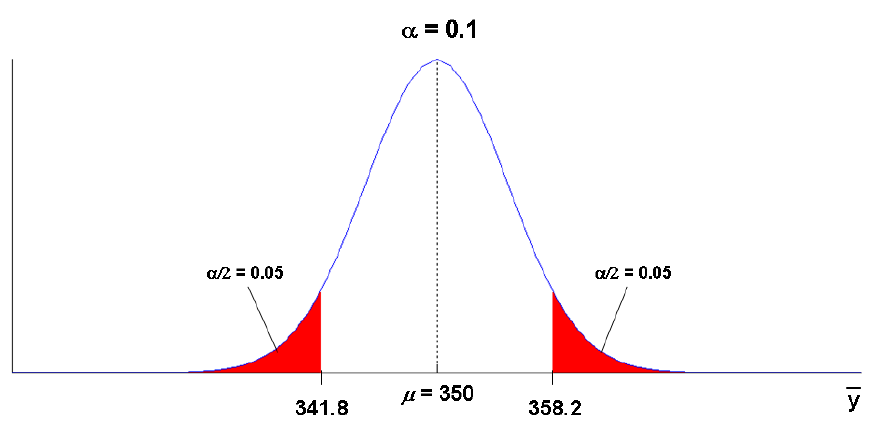
\includegraphics[width=0.6\textwidth]{img/normaldist}
\end{frame}


\begin{frame}
  \frametitle{Statistical Hypothesis (3)}

  \begin{block}{Defining the Null Hypothesis}
    \begin{itemize}
    \item Previous knowledge about the process (to find out if there
      was a change in the parameter);
    \item Values obtained from theory or models (validation of the
      model);
    \item Requirements of a project (conformity tests);
    \end{itemize}
  \end{block}
  \medskip

  \begin{block}{Hypothesis Test}
    \begin{itemize}
    \item Obtain the sampled data;
    \item Calculate the test statistics;
    \item Make a decision based on the value found;
    \end{itemize}
  \end{block}
\end{frame}

\begin{frame}
  \frametitle{Statistical Hypothesis (example)}
    \begin{columns}[c]
      \column{0.8\textwidth}
      \begin{itemize}
      \item We define a null hypothesis as ``the cans have an
        average of 350ml of beer in it.'';
        \begin{equation*}
          H_0 : \mu = 350ml
        \end{equation*}
        \begin{equation*}
          H_a : \mu \neq 350ml
        \end{equation*}
      \item We take a sample of 20 cans, and measure the contents of each;
      \item The sample average $\bar{y}$ is an estimator for the
        population's mean $\mu$;
        \begin{itemize}
          \item if $\bar{y} = 350$, the null hypothesis is not refuted;
          \item if $\bar{y} \neq 350$, the null hypothesis is refuted
            - the reason must be studied.
          \item this is the statistic we want to test;
        \end{itemize}
      \end{itemize}
      \column{0.2\textwidth}
      
\includegraphics[width=1\textwidth]{img/duff}
    \end{columns}
\end{frame}

\begin{frame}
  \frametitle{Statistical Hypothesis (example - 2)}
  \begin{block}{The alternate hypothesis}
    \begin{itemize}
    \item $\bar{y}$ can assume a range of values;
    \item Thus, we define the $H_a$ as a range of values different
      from $H_0$;
    \end{itemize}
  \end{block}
  \bigskip
  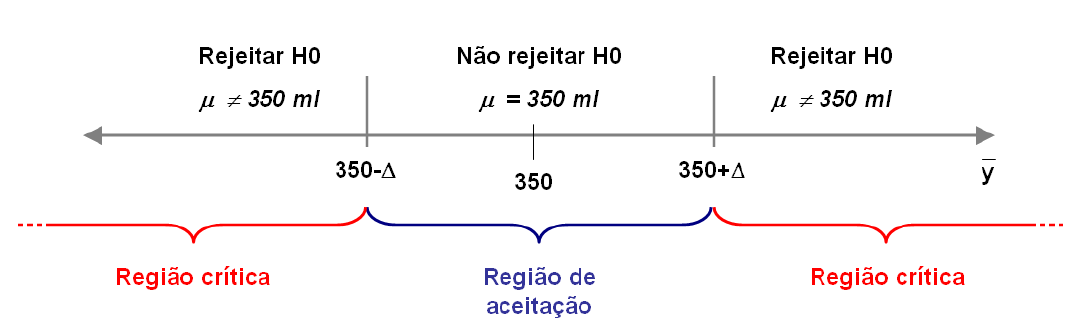
\includegraphics[width=0.8\textwidth]{img/criticalregion}
\end{frame}

\begin{frame}
  \frametitle{Errors in Hypothesis Tests}
  
  \begin{center}
    \begin{tabular}{ccc}
      \hline
      Decision & $H_0$ is True & $H_0$ is False\\
      \hline
      Fail to Reject $H_0$ & no error & type II error\\
      Reject $H_0$ & type I error & no error\\
      \hline
    \end{tabular}
  \end{center}
  
  \bigskip

  \begin{itemize}
    \item Type I error (False positive): rejecting the null hypothesis
      when it is true; \only<2>{\alert{We don't want this!}}
    \item Type II error (False negative): not rejecting the null
      hypothesis when it is false;
  \end{itemize}
\end{frame}

\begin{frame}
  \frametitle{Significance Level}

  \begin{block}{}
    Significance levels are the probabilities for one of the errors to happen:
    \begin{itemize}
    \item \structure{$\alpha$}: \alert<2>{Probability of a type I error;}
    \item \structure{$\beta$}: \alert<3>{Probability of a type II error;}
    \end{itemize}
  \end{block}

  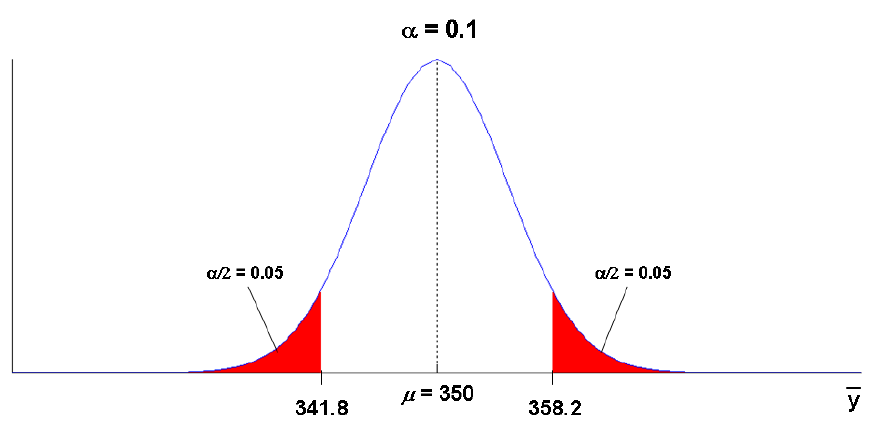
\includegraphics[width=0.6\textwidth]{img/normaldist}

  \begin{block}{}
    \only<1>{The probability distribution above are possible values for the
    \structure{population mean}.}
    \only<2>{The probability of the population mean to fall in the defined critical area}
    \only<3>{Statistically, we can change the statistic by changing
      the sample size and the confidence interval}
  \end{block}
\end{frame}

\begin{frame}
  \frametitle{Things to keep in mind about statistical errors}
  \begin{itemize}
    \item Type I errors depends only on the probability distribution
      of the null hypothesis - easier to control;
    \item Type II errors depends on the true value of the parameter
      under study; Harder to specify and control;
    \item Rejecting $H_0$ - Strong conclusion;
    \item Not rejecting $H_0$ - weak conclusion
      \begin{itemize}
        \item In particular, Not rejecting $H_0$ is {\it NOT} evidence
          towards $H_0$;
      \end{itemize}
  \end{itemize}
\end{frame}


\subsection{General Procedure}

\begin{frame}
  \frametitle{General Procedure for an hypothesis Test}
  \begin{itemize}
    \item Identify the parameter that interests us;
    \item Define $H_0$
    \item Define $H_A$, decide whether it is one or two sided;
    \item Determine the confidence level $\alpha$;
    \item Determine which statistical test to use;
    \item Decide the critical region of the test (parameter values);
    \item Calculate the statistics;
    \item Reject, or not reject $H_0$;
  \end{itemize}
\end{frame}

\subsection{case studies}

\begin{frame}
  \frametitle{Case: Normal Distribution; Known Variance (1)}
  \begin{equation*}
    H_0 : \mu = \mu_0 
  \end{equation*}
  \begin{equation*}
    H_A : \mu \neq \mu_0
  \end{equation*}

  \begin{itemize}
  \item Desired significance level: $\alpha = 0.05$
  \item The sample distribution of $\bar{y}$ is normal, with variance
    $\sigma^2/n$;\\ ($\bar{y}$ is an estimation of $\mu$);
  \item If $H_0$ is true, $\bar{y} ~ N(\mu_0,\sigma^4/n)$;
  \end{itemize}
\end{frame}

\begin{frame}
  \frametitle{Case: Normal Distribution; Known Variance (2)}
  \begin{itemize}
  \item Standardization of the sample mean:
    \begin{equation*}
      Z_o = \frac{\bar{y} - \mu_0}{\sigma/\sqrt{n}}
    \end{equation*}
  \item If $H_0$ is true, $Z_0$ will fall in $N(0,1)$
  \item Probability $(1 - \alpha)$ of $Z_0$ falling in the interval
    $-Z_{\alpha/2} +Z_{\alpha/2}$
    \begin{itemize}
      \item $Z_{\alpha/2}$ is the $100(1-\alpha/2)$ of a normal distribution.
      \item This is for a two-sided test.
    \end{itemize}
  \end{itemize}
\end{frame}

\begin{frame}
  \frametitle{Case: Normal Distribution; Known Variance (3)}
  \begin{itemize}
  \item If $z_0 < -z_{\alpha/2}$ or $z_0 > z_{\alpha/2}$, then reject
    $H_0$ with significance level $\alpha$
  \item If $-z_{\alpha/2} < z_0 < z_{\alpha/2}$, then do no reject $H_0$
  \end{itemize}
  \bigskip

  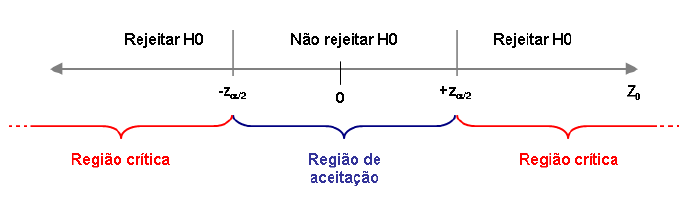
\includegraphics[width=0.7\textwidth]{img/criticalregionZ}
\end{frame}

\begin{frame}[fragile,singleslide]
  \frametitle{Case: Normal Distribution; Known Variance (4)}
  \begin{itemize}
    \item Let's assume $\bar{y} = 359.6ml, n = 20, \sigma = 22ml$\\

      \begin{equation*}
        z_0 = \frac{359.6 - 350}{22/\sqrt{20}} = 1.962
      \end{equation*}
      \bigskip

    \item The critical values of the Z test for $\alpha = 0.05$ are $1.96$

    \item Since $z_0 > 1.96$ there is enough evidence to reject the
      null hypothesis.
  \end{itemize}
\begin{block}{}
{\smaller
\begin{verbatim}
> library(TeachingDemos)
> samples<-c(373, 346, 357, 322, 382, 365, 390, 349, 366, 402, 
  344, 353, 377, 355, 345, 360, 356, 316, 365, 379)
> (r.test(samples, mu=350, sd=22, alternatives, "two.sided",
     conf.level = 0.95))
\end{verbatim}}
\end{block}
\end{frame}

\begin{frame}
  \frametitle{Case: Normal Distribution; Unknown Variance (1)}
  \begin{block}{}
    The Z test had some assumptions about the population
    (distribution, variance). When those assumptions don't hold, we
    need to adapt the test accordingly.
  \end{block}
  
  \begin{equation*}
    H_0 : \mu = \mu_0
  \end{equation*}
  \begin{equation*}
    H_A : \mu < \mu_0
  \end{equation*}
  
  \begin{itemize}
    \item Desired significance level: $\alpha = 0.01$
    \item Sample Variance: $S^2$. Used as an estimator for $\sigma^2$
    \item If $H_0$ is true, then
      \begin{equation*}
        T_0 = \frac{\bar{y} - \mu_0}{S/\sqrt{n}}
      \end{equation*}
      follows a $t_{n-1}$ probability distribution (different from N!)   
  \end{itemize}
\end{frame}

\begin{frame}[fragile,singleslide]
  \frametitle{Case: Normal Distribution; Unknow Variance (2)}

  \begin{itemize}
  \item Assume $\bar{y} = 343.1$ml, n = 29, s = 18.2ml:
    \begin{equation*}
      t_0 = \frac{343.1 - 350}{18.2/\sqrt{20}} = -1.69
    \end{equation*}
  \item Critical value for the test: $-t_{0.01,19} = -2.54;$\\

  \item Because the value for the statistical test is not lower than
    the critical value, we conclude that the evidence is insufficient
    to reject $H_0$, at the 99\% significance level.    
  \end{itemize}

  \begin{block}{}
    {\smaller
\begin{verbatim}
> samples<-c(365,318,341,340,309,368,344,346,330,
  382,346,338,328,334,349,358,365,318,342)
> (t.test(samples, alternative = "less", mu = 350,
  conf.level = 0.99))
\end{verbatim}}
  \end{block}
\end{frame}

\subsection{PValues}

\begin{frame}
  \frametitle{Our Results so far}
  \begin{itemize}
  \item The result of a Hypothesis test, as we have done them so far, will say that:
    \begin{block}{}
      ``The evidence is enough/not enough to reject $H_0$, with
      significance level $\alpha$.''
    \end{block}
    \medskip
  \item This is actually not really useful to judge an experiment:
    \begin{itemize}
    \item Does not offer the exact value of the test statistic (how close is it to $\alpha$?)
    \item Fixes the significance level beforehand.
    \end{itemize}
  \end{itemize}
\end{frame}

\begin{frame}
  \frametitle{The P-Value!}

  \begin{block}{P-Value}
    The minimum significance level that would result in the rejection
    of $H_0$ for the given data.
  \end{block}
  \bigskip
  
  In other words...
  \bigskip

  \begin{block}{P-Value}
    Probability that the test statistic will assume a value more
    extreme than the observed, if $H_0$ is true (probability of a
    Type I error).
  \end{block}
\end{frame}

\begin{frame}
  \frametitle{P-Value (2)}
  \begin{itemize}
  \item Example: in the last case, for $t_0 = -1.84$, the p-value would be:
    \begin{equation*}
      p = P(t_0 \leq -1.84|H_0) = \int^{-1.84}_{\infty} t_{19}dy = 0.041
    \end{equation*}
  \item The null hypothesis would be rejected for any $\alpha > 0.041$;
    \medskip

  \item We still need to define an {\it a priori} desired significance level!    
  \end{itemize}
\end{frame}

\begin{frame}
  \frametitle{Reality Check Time!}
  ``pvaluecomic.jpg''
\end{frame}

\begin{frame}
  \frametitle{P-value and magnitude}
  
  \begin{block}{Another issue with P values}
    We can calculate an arbitrarily low P value by choosing a large enough $n$.
    \medskip
    
    ... and this is easy to do in computer sciences!
  \end{block}
  
  \begin{block}{Example: n = 5000, $\bar{y}$ = 349ml, s = 21ml}
    \begin{itemize}
      \item $t_0 = -3.36$
      \item $p = 3.93 x 10^{-4}$
    \end{itemize}
  \end{block}
\end{frame}

\begin{frame}
  \frametitle{P-value and magnitude}

  \begin{block}{}
    So, we need to use estimators for the effect's magnitude, along
    with tests for statistical significance.
  \end{block}
  \begin{itemize}
  \item Simple difference: $\bar{y} - \mu_0$
  \item Cohen's $d$: 
    \begin{equation*}
      d = \frac{\bar{y} - \mu_0}{s}
    \end{equation*}
  \item Bootstrap estimators;    
  \end{itemize}
\end{frame}


\end{document}
